\chapter{An Approach for Reproducible Analysis}

A strategy is needed to facilitate reproducibility of NMR data analysis.
This chapter will describe in more detail the common characteristics of
the missing data and what role they play as well as why it is important to
capture them, a model for capturing that data, and a strategy for using
the model during the analysis process.


\section{Missing data and its role in analysis}

% need to cover what the data is, how it plays a role in NMR analysis, 
% why it's important to capture
As was described in earlier sections, 
spectral analysis, including peak picking, GSS construction, GSS and resonance
typing, sequential GSS assignment, and sequence-specific GSS assignment is 
accomplished using a step-by-step process of deductive reasoning 
which is often augmented by computational tools.  The computational 
results may be subject to manual validation, correction, and extension
\cite{guerry2011automated}.  This section will explore the various types
of data involved.

\subsection{Intermediate results}
An important feature of the analysis process is that the final results are
not the output of a single replicable step, but rather of a series of steps
of refinement and modification.  Thus, the analysis process implicitly 
generates a new data set (from the previous one) after every modification, 
whether manual or automated.

Implicit in the sequence of data sets are logical dependencies of derived
data upon features of the previous data set: the context of each deduction
is important, because the exact context determines what deductions may be
made and the confidence level of each deduction. % TODO an example

The importance of capturing intermediates is due to the dependence of 
deductions on context: without knowing the context, it is impossible to 
evaluate the correctness, confidence, and alternative interpretations of
a deduction.  In standard approaches to analysis, the contexts are not
captured; they are implicit.  By making the contexts explicit, it becomes
possible not only to fully recapitulate the process of analysis, but also 
to employ error detection and correction strategies by analysis
of deductions and their contexts.  
An interesting side-effect of capturing
contexts is that analysis can be restarted in the middle, by selecting an
appropriate context and applying a different deduction.

% TODO
% come up with a simple example that demonstrates: 
%   1) the dependence of deductive ability on context
%   2) the concept and utility of multiple snapshots
%   3) the concept and utility of tracking logical dependencies

\subsection{Deductive reasoning}
As was covered earlier, the deductive process of reasoning which plays
a major role in data analysis generates intermediate data sets.  Associated
with the generation of these data sets is a rule employed for deduction.

% TODO do I need to say something about the proposed library of deductive reasons? or does that come later?
Each rule is an embodiment of NMR-specific knowledge of how to interpret a
data feature.  In general, a deductive rule requires an input, produces an
output, and has an intuitive justification for its action.  
% TODO example

Application of these rules provides a rationale for manual modifications.  The
rationale is a justification that the change modification is correct, as
well as an indication of why the change was made.  Therefore, capturing the
deductive rules employed enables verification of the veracity of modifications. 
It also facilitates knowledge transfer, both in the contexts of collaboration
and teaching, by providing a meaningful annotation (with reference to the
domain of NMR) for actions taken.

\subsection{Extraneous Results}
During analysis, some portion of the positive results are not of direct interest
to the final answer.  Not only peaks, but also resonances and GSSs are included.
The positive results include both false positives, caused by noise or
artifacts, and true positives, caused by contaminants.

Although not of direct interest, such extraneous results play a role in 
the process of analysis: as was covered earlier, when making a manual
modification, a deductive rule is applied to a context (data set).  Changing 
the context affects which rules apply and what deductions are made; 
therefore, as a part of the context, extraneous results matter during analysis. 
If incorrectly identified or left unrecognized, extraneous features can
lead to incorrect peak picking, chemical shift assignments, GSSs, and GSS
assignments.

A further benefit of capturing extraneous results is the ability to distinguish
between identifying a data feature and interpreting it.  In other words, peaks
picked during peak picking are treated as positives, this is the "identification"
phase; in the later "interpretation" phase, these peaks are separated into
false positives and true positives.  This allows rectification of the 
discrepancies between uncorrected computational results and the final,
deposited results as well as marking potentially suspicious results for 
future perusal.  It should also be noted that picking a peak, then
interpreting it as extraneous and discarding it is typically not reported in
final data sets, despite containing important information.
There is a balance between false positives and false negatives \cite{pine};
false negatives are more undesirable \cite{pine, saga, guntert2009automated},
and capturing extraneous results helps to avoid this tradeoff: by reducing
the cost of a false positive, tools are free to focus on avoiding false
negatives.

The process of separating positives into false and true is prone to 
introducing bias; by keeping and reporting the initial results, such bias
can be estimated.  This is not possible if the extraneous results are not
reported, and also allows the feature identification phase to proceed
without bias, since error correction will be applied at a later stage. 
By providing additional context, it may be possible to estimate the quality 
of an analysis, where errors may be most likely found in the borderline 
cases; it will also help assigning confidence levels to datums by not.
Additional quality measures enabled include the number of peaks found by the
peak-picker, the number of false positives, the number of peaks assigned to
GSSs, and the number of GSSs assigned to residues.  It may also be possible
to estimate contamination, incompleteness and overcompleteness, overfitting, 
and consistency.

\subsection{Notes}
Due to the difficulties inherent in data analysis, situations are reached
in which the interpretation of a specific feature is problematic:
\begin{itemize}
  \item uncertain or impossible.  The evidence for a particular deduction 
    is not solid.
  \item ambiguous.  Multiple interpretations of a feature are consistent
    with the data and satisfy the constraints.  It is not possible to choose
    between them.
  \item inconsistent.  The data set is in an inconsistent state, or a 
    deduction would leave it in an inconsistent state.
\end{itemize}
A simple example is non-stereospecific sidechain proton assignments: 
a residue such as a Histidine or Lysine which has two beta protons will 
often give rise to two resonances, one for each beta proton; however, 
without additional information, it is impossible to assign a resonance to
a specific atom.  A related example is caused by the two delta and epsilon
protons in Phenylalanine and Tyrosine aromatic sidechains; the two resonances,
even if distinguishable, can not be uniquely assigned to atoms.  In both
cases, the ambiguity is resolvable through the use of additional information;
however, before that additional information is provided, it is useful to be
able to store what is known -- that there are two peaks, each of which 
corresonds to one atom, but exactly which is unsure -- as an indication to
future analysis or perusal that a problem has been identified but not yet
solved.

The key idea is, given the inevitability of such problems during data
analysis, to create facilities for explicitly recognizing, discussing, 
and handling such problems \cite{robillard2007concerns}. 
Several strategies for such an approach 
are covered in \cite{nuseibeh2000inconsistency} including deferral of the
problem while flagging it for later follow-up.

Enabling the representation of such data has similarities to the probabilistic
approach applied by PINE \cite{pine} to great effect.  
PINE deals with the innate uncertainty of data 
analysis by resolving the tradeoff between false positives and false 
negatives through association of a probabilistic confidence metric with each
feature interpretation; low confidence values are used as evidence that an
interpretation is suspicious and needs additional verification or data.
In a complementary approach, capturing notes of analysis issues also 
resolves the tradeoff for manual analysis, by enabling the association of
an explanatory or warning message with suspected low-quality deductions.
In addition, the message may contain more information than a scalar: it may
necessarily refer to multiple conflicting pieces of the data set in the case
of a contradiction.

\subsubsection{Example}
peak pick overlapped peaks, not knowing actual extent of overlap (if any)

\subsubsection{Example}
multiple matching sequential GSSs


\section{A Model for Reproducible NMR}

\subsection{Data models}
A data model is a means of specifying the structure of information  
\cite{codd1970relational}.  This
information may be used as inputs and outputs for computational tools, or
it may be archived and available for reference use.  Data models are useful
because they provide a formal specification of the structure, which enables
unambiguous, correct, and automated use of data.  Data models are
abstract specifications; they must be implemented in source code in order
to become a usable artifact.

In the field of NMR, both the BMRB \cite{bmrb} and CCPN \cite{ccpn} have
created descriptive, extensive and useful data models, and have implemented them 
in programs and as Application Programming Interfaces (APIs).  These are used
by additional programs to help manage the exchange of data with external
programs.

This section will cover a data model for reproducibility.  Once a data
model exists, it can be implemented as part of a software program that
facilitates reproducible data analysis, as will be covered in a later 
chapter.  The core of this data model is formed by the BMRB \cite{bmrb}
and CCPN \cite{ccpn} data models.  These models are then extended with
several additional data types and properties in order to enable 
reproducibility.

\subsection{Intermediate results}
The strategy for modelling intermediate results is based on the data models
of existing version control systems, including Git \cite{loeliger2012git},
SVN \cite{svn}, and CVS \cite{cvs}.  Figure-\ref{intermediates} shows the
general properties of the solution: a sequence of snapshots of the data set,
where associated with each snapshot is a small amount of metadata:
\begin{itemize}
 \item timestamp
 \item author
 \item parent, or previous snapshot.  This maintains the order of the 
  snapshots
\end{itemize}

When multiple snapshots are captured, they can be compared as in Figure-\ref{diff},
and also can be used to track logical dependencies of analysis.

Figure-\ref{snapshot_model} shows an entity-relationship (ER) model built
using MySQLWorkbench.

\subsection{Deductive reasoning}
 - a library of reasons, each including:
   - a meaningful name
   - an explanation of its meaning within the NMR domain
   - intended use
   - intended result
   - examples as picture
 - reasons are applied to annotate intermediate results
\subsubsection{Example}
present most or all of the library, in picture and textual format

\subsection{Extraneous results}
 - extend BMRB and CCPN models
 - for peaks, resonances, GSSs:
   - add data fields
   - track category
   - during analysis, never delete these.  always "soft delete" by changing category
\subsubsection{Example}
CCPN peak pick as initial peak list, then corrections I made as peak list 
where each peak has additional fields

\subsection{Notes}
 - extend BMRB and CCPN models
 - note, which can refer to any other datum
\subsubsection{Example}
odd feature in data, unable to resolve


\section{An Implementation of the Model}


\section{Applying Reproducible Analysis}
 - what to do -- tips and suggestions to be effective
 - what not to do -- common roadblocks and problems
% maybe talk about the culture of the lab notebook?
% could this belong in its own chapter?
% or in the software chapter, or in the 'reproducible data sets' chapter?


\section{Archiving Reproducible Data Sets}
 - the NMR-Star file format, my parser, and others
 - the usefulness of NMR-Star files
 - the NMR-Star data dictionary
 - extending the NMR-Star data dic
 - other efforts to provide this NMR-Star integration ???


\section{Discussion}
 - lab notebooks
 - what data is missing
 - extending existing models to support these data
 - getting a handle on bias of data analysis
 - making things explicit


\section{Conclusion}
 - could go in with previous section


% figures
\clearpage
\section{Figures}

\begin{figure}[h]
  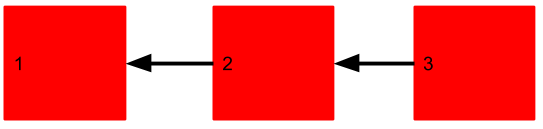
\includegraphics[scale=0.5]{figures/intermediates}
  \caption{Intermediate data sets form a linked chain.}
  \label{intermediates}
\end{figure}

\begin{figure}
  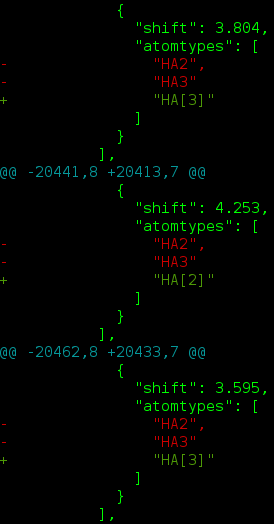
\includegraphics[scale=0.5]{figures/diff}
  \caption{Capturing intermediates allows comparison, such as diffs.}
  \label{diff}
\end{figure}

\begin{figure}
  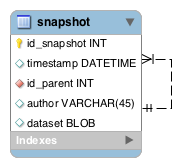
\includegraphics[scale=0.5]{figures/snapshot_model}
  \caption{A relational model of a snapshot.}
  \label{snapshot_model}
\end{figure}

\begin{figure}
  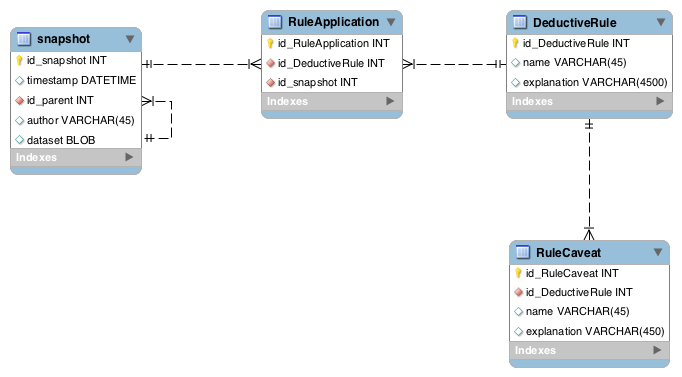
\includegraphics[scale=0.5]{figures/deduction_model}
  \caption{A relational model of a snapshot and deductions.}
  \label{deduction_model}
\end{figure}

